% The following sections are part of the front matter, but are not generated
% automatically by LaTeX; the use of \chapter* means they are not numbered.

% -----------------------------------------------------------------------------

\chapter*{Executive Summary}

% {\bf A compulsory section, of at most $1$ page} 
% \vspace{1cm} 

% \noindent
% This section should pr\'{e}cis the project context, aims and objectives,
% and main contributions (e.g., deliverables) and achievements; the same 
% section may be called an abstract elsewhere.  The goal is to ensure the 
% reader is clear about what the topic is, what you have done within this 
% topic, {\em and} what your view of the outcome is.

% The former aspects should be guided by your specification: essentially 
% this section is a (very) short version of what is typically the first 
% chapter.  Note that for research-type projects, this {\bf must} include 
% a clear research hypothesis.  This will obviously differ significantly
% for each project, but an example might be as follows:

% \begin{quote}
% My research hypothesis is that a suitable genetic algorithm will yield
% more accurate results (when applied to the standard ACME data set) than 
% the algorithm proposed by Jones and Smith, while also executing in less
% time.
% \end{quote}

% \noindent
% The latter aspects should (ideally) be presented as a concise, factual 
% bullet point list.  Again the points will differ for each project, but 
% an might be as follows:

% \begin{quote}
% \noindent
% \begin{itemize}
% \item I spent $120$ hours collecting material on and learning about the 
%       Java garbage-collection sub-system. 
% \item I wrote a total of $5000$ lines of source code, comprising a Linux 
%       device driver for a robot (in C) and a GUI (in Java) that is 
%       used to control it.
% \item I designed a new algorithm for computing the non-linear mapping 
%       from A-space to B-space using a genetic algorithm, see page $17$.
% \item I implemented a version of the algorithm proposed by Jones and 
%       Smith in [6], see page $12$, corrected a mistake in it, and 
%       compared the results with several alternatives.
% \end{itemize}
% \end{quote}

This project is concerned with the use of deep learning to automate the calculation of the amount of annual skeletal matter produced by corals.

First, the process of labelling density bands present in two dimensional slices is automated. This is achieved using a convolutional neural network based off of the U-Net architecture~\cite{ronneberger2015u}. To train this network, a dataset containing ${\sim}600$ images was curated from slices extracted from seven individual coral samples. Various data augmentation techniques were also used to artificially expand the dataset. To measure performance, an accuracy metric based off of the Hausdorff distance between the predicted and ground truth boundaries is used. This initial architecture achieved an average Hausdorff distance of 1.X pixels.

Second, the process of labelling density bands present in three dimensions is automated. To this end, the U-Net architecture is modified to process three dimensional data. A larger dataset of manually labelled adjacent slices was curated to train this network containing ${\sim}X$ images extracted from $X$ coral samples. This architecture making use of the third dimension achieved an average Hausdorff distance of X pixels.

Finally, once the density bands are identified, the process of calculating the volume of skeletal matter produced annually is automated using various techniques.

\begin{itemize}
    \item I spent 25 hours manually labelling coral data.
    \item I generated a 2D dataset containing ${\sim}600$ images and a 3D dataset containing ${\sim}X$ images using various scripts I wrote.
    \item Having not taken the ``Deep Learning'' unit, I spent 20 hours researching and learning about the field of deep learning.
    \item I learned how to use the Keras and TensorFlow libraries in order to implement the networks used.
    \item I modified an existing 2D U-Net implementation and trained it on the curated dataset.
    \item I extended the U-Net architecture to process 3D data.
    \item I wrote a ``data generator'' from scratch in Python to allow the input of 3D data into the network since Keras does not have its own implementation.
    \item I implemented online data augmentation of the 3D data.
    \item I implemented a custom accuracy metric in C and wrapped it in a Python function to achieve a ${\sim}625$ times speed up allowing the accuracy to be calculated in minutes rather than days.
    \item I performed hyper parameter optimisation in order to maximise the performance achieved by the various architectures.
\end{itemize}

% -----------------------------------------------------------------------------

% \chapter*{Summary of Changes}

% {\bf A conditional section, of at most $1$ page} 
% \vspace{1cm} 

% Iff. the dissertation represents a resubmission (e.g., as the result of
% a resit), this section is compulsory: the content should summarise all
% non-trivial changes made to the initial submission.  Otherwise you can
% omit it, since a summary of this type is clearly nonsensical.

% When included, the section will ideally be used to highlight additional
% work completed, and address criticism raised in any associated feedback.
% Clearly it is difficult to give generic advice about how to do so, but
% an example might be as follows:

% \begin{quote}
% \noindent
% \begin{itemize}
% \item Feedback from the initial submission criticised the design and 
%       implementation of my genetic algorithm, stating ``there seems 
%       to have been no attention to computational complexity during the
%       design, and obvious methods of optimisation are missing within
%       the resulting implementation''.  Chapter $3$ now includes a
%       comprehensive analysis of the algorithm, in terms of both time
%       and space.  While I have not altered the algorithm itself, I
%       have included a cache mechanism (also detailed in Chapter $3$)
%       that provides a significant improvement in average run-time.
% \item I added a feature in my implementation to allow automatic rather
%       than manual selection of various parameters; the experimental
%       results in Chapter $4$ have been updated to reflect this.
% \item Questions after the presentation highlighted a range of related
%       work that I had not considered: I have make a number of updates 
%       to Chapter $2$, resolving this issue.
% \end{itemize}
% \end{quote}

% -----------------------------------------------------------------------------

\chapter*{Supporting Technologies}

% {\bf A compulsory section, of at most $1$ page}
% \vspace{1cm} 

% \noindent
% This section should present a detailed summary, in bullet point form, 
% of any third-party resources (e.g., hardware and software components) 
% used during the project.  Use of such resources is always perfectly 
% acceptable: the goal of this section is simply to be clear about how
% and where they are used, so that a clear assessment of your work can
% result.  The content can focus on the project topic itself (rather,
% for example, than including ``I used \mbox{\LaTeX} to prepare my 
% dissertation''); an example is as follows:

% \begin{quote}
% \noindent
% \begin{itemize}
% \item I used the Java {\tt BigInteger} class to support my implementation 
%       of RSA.
% \item I used a parts of the OpenCV computer vision library to capture 
%       images from a camera, and for various standard operations (e.g., 
%       threshold, edge detection).
% \item I used an FPGA device supplied by the Department, and altered it 
%       to support an open-source UART core obtained from 
%       \url{http://opencores.org/}.
% \item The web-interface component of my system was implemented by 
%       extending the open-source WordPress software available from
%       \url{http://wordpress.org/}.
% \end{itemize}
% \end{quote}

\begin{itemize}
\item Avizo
\item GIMP
\item Keras
\item TensorFlow
\item OpenCV
\item Isambard
\item BlueCrystal Phase 4
\end{itemize}

% -----------------------------------------------------------------------------

\chapter*{Notation and Acronyms}

\begin{tabular}{lcl}
ANN                 &:     & Artificial Neural Network \\
CNN                 &:     & Convolutional Neural Network \\
SGD                 &:     & Stochastic Gradient Descent \\
\end{tabular}

% -----------------------------------------------------------------------------

\chapter*{Acknowledgements}

I am extremely grateful to Dr. Tilo Burghardt whose enthusiasm, support, and guidance throughout this project has been invaluable. His passion for education is incredible and I will forever be thankful for his contributions throughout my entire degree. I would also like to extend my sincere thanks to Dr. Erica Hendy and Dr. Kenneth Johnson for their expertise and enthusiasm for the project. I am also grateful to Leonardo for the time and effort he put into labelling data for this project as well as his consistent support throughout.

% =============================================================================

% After the front matter comes a number of chapters; under each chapter,
% sections, subsections and even subsubsections are permissible.  The
% pages in this part are numbered with Arabic numerals.  Note that:
%
% - A reference point can be marked using \label{XXX}, and then later
%   referred to via \ref{XXX}; for example Chapter\ref{chap:context}.
% - The chapters are presented here in one file; this can become hard
%   to manage.  An alternative is to save the content in seprate files
%   the use \input{XXX} to import it, which acts like the #include
%   directive in C.

\mainmatter

% -----------------------------------------------------------------------------

\chapter{Contextual Background}
\label{chap:context}

This chapter outlines and motivates the main objectives of the project. First, the importance of the analysis of corals is discussed. Next, the motivations for an automated process of analysis are outlined and the choice of a deep learning based solution is discussed. Finally, related works in the analysis of corals are highlighted and briefly discussed.

\section{Introduction}

\subsection{Corals}

Introduce coral density bands cite showing they exist. Explain what they can be useful for.

\section{Motivations}

\subsection{Manual Processing}

Explain the current method that erica and co use to calculate what we are trying to calculate. Introduce the density of coral?

\subsection{Dataset}

Introduce the dataset (whats the name? can use it in the subsection name).

\subsection{Image Segmentation}

Why are we using deep learning for it? why is it an important area of research?
Introduce image segmentation. Mention U-Net and SegNet are used for this and are discussed in tech bg. Mention that unet is often used for biomedical data for example cells etc and it was in interesting experiment applying it to volumetric ct scans of coral skeletons.

\section{Related Work}

% {\bf A compulsory chapter,     of roughly $5$ pages}
% \vspace{1cm} 

% \noindent
% This chapter should describe the project context, and motivate each of
% the proposed aims and objectives.  Ideally, it is written at a fairly 
% high-level, and easily understood by a reader who is technically 
% competent but not an expert in the topic itself.

% In short, the goal is to answer three questions for the reader.  First, 
% what is the project topic, or problem being investigated?  Second, why 
% is the topic important, or rather why should the reader care about it?  
% For example, why there is a need for this project (e.g., lack of similar 
% software or deficiency in existing software), who will benefit from the 
% project and in what way (e.g., end-users, or software developers) what 
% work does the project build on and why is the selected approach either
% important and/or interesting (e.g., fills a gap in literature, applies
% results from another field to a new problem).  Finally, what are the 
% central challenges involved and why are they significant? 
 
% The chapter should conclude with a concise bullet point list that 
% summarises the aims and objectives.  For example:

% \begin{quote}
% \noindent
% The high-level objective of this project is to reduce the performance 
% gap between hardware and software implementations of modular arithmetic.  
% More specifically, the concrete aims are:

% \begin{enumerate}
% \item Research and survey literature on public-key cryptography and
%       identify the state of the art in exponentiation algorithms.
% \item Improve the state of the art algorithm so that it can be used
%       in an effective and flexible way on constrained devices.
% \item Implement a framework for describing exponentiation algorithms
%       and populate it with suitable examples from the literature on 
%       an ARM7 platform.
% \item Use the framework to perform a study of algorithm performance
%       in terms of time and space, and show the proposed improvements
%       are worthwhile.
% \end{enumerate}
% \end{quote}

\section{Summary of Objectives}

The main objective of this project is to automate the calculation of annual skeletal matter produced by corals. This objective is broken down into multiple tasks:

\begin{enumerate}
    \item Curate a dataset of image-label pairs from the raw unlabelled dataset provided to us.
    \item Train an existing two dimensional neural network architecture to extract the annual density boundaries present in the data.
    \item Modify the architecture to process three dimensional data.
    \item Conceive and implement an accuracy metric to assess the performance of different networks on the data.
    \item Optimise hyper parameters of the chosen network architecture to maximise accuracy.
    \item Make use of these extracted boundaries to automate the calculation of the annual skeletal matter produced.
    \item Package the implementation in a form usable by researchers at the Natural History Museum and the School of Earth Sciences at the University of Bristol.
\end{enumerate}

% -----------------------------------------------------------------------------

\chapter{Technical Background}
\label{chap:technical}

% {\bf A compulsory chapter,     of roughly $10$ pages} 
% \vspace{1cm} 

% \noindent
% This chapter is intended to describe the technical basis on which execution
% of the project depends.  The goal is to provide a detailed explanation of
% the specific problem at hand, and existing work that is relevant (e.g., an
% existing algorithm that you use, alternative solutions proposed, supporting
% technologies).  

% Per the same advice in the handbook, note there is a subtly difference from
% this and a full-blown literature review (or survey).  The latter might try
% to capture and organise (e.g., categorise somehow) {\em all} related work,
% potentially offering meta-analysis, whereas here the goal is simple to
% ensure the dissertation is self-contained.  Put another way, after reading 
% this chapter a non-expert reader should have obtained enough background to 
% understand what {\em you} have done (by reading subsequent sections), then 
% accurately assess your work.  You might view an additional goal as giving 
% the reader confidence that you are able to absorb, understand and clearly 
% communicate highly technical material.

As outlined in Chapter \ref{chap:context}, the objective of this project is to use deep learning to automate the calculation of the amount of skeletal matter produced by corals annually. This chapter introduces and briefly describes the techniques used in order to achieve this goal.

\section{Deep Learning}

Based loosely on the structure of the brain, artificial neural networks (ANNs) are computational models that have proved useful in a wide range of applications~\cite{lecun2015deep, healthcare, nlp}\textemdash a notable example being the recent success of convolutional neural networks in the field of computer vision~\cite{compvision, semanticseg}. Deep learning is a form of machine learning that concerns the use of ANNs with many layers\textemdash hence the name ``deep'' learning. The field has seen a significant increase in popularity in recent years since a network named AlexNet famously won the ImageNet Large Scale Visual Recognition Challenge in 2012\footnote{\url{http://www.image-net.org/challenges/LSVRC/2012/results.html}}, performing considerably better than the previous state-of-the-art~\cite{alexnet}.

A typical fully connected ANN is a layered network of ``neurons'' connected by a series of ``weights''. A neuron is simply an object that produces a weighted sum of some number of inputs. This weighted sum is often passed through a non-linear ``activation'' function and the final result is referred to as the ``activation'' of the neuron. When values are supplied to the input neurons of the network, these values are forward-propagated through the network, activating each layer of neurons which, in turn, activate the next layer. The resulting activations of the neurons in the final layer are the output of the network.

\subsection{Convolutional Neural Networks}

The convolutional neural network (CNN) is a type of neural network named after the discrete convolution operation that sets these models apart from typical fully connected ANNs. The convolution operation makes use of surrounding pixels in order to change the value of a central pixel. The 2D discrete convolution operation is defined as

\begin{equation}
    g(x,y)=\sum_{i=1}^{m}\sum_{j=1}^{n}f(x-j,y-k)h(j,k)
\end{equation}

\noindent
where $f$ is the input image, $h$ is an $m\times n$ kernel, and $g$ is the resulting image.

CNNs often contain multiple convolutional layers in which increasingly complex features of an image may be detected by making use of a combination of simpler features detected in previous layers. A convolutional layer convolves the channels of an image with multiple learned kernels. A channel is simply a component of an image\textemdash an RGB image, for example, consists of three channels, whilst a greyscale image consists of only one. The output of these operations will be multiple modified images that are referred to as ``feature maps''. These feature maps can then be used as the input channels to the next layer, and so on.

As well as the convolution operation, the max-pooling operation is often used. The max-pooling operation is used to decrease the dimensionality of the input in attempt to force the network to ``learn'' features present in the input. These operations are illustrated in Figure \ref{fig:operations}.

\begin{figure}[t]
    \centering
    \begin{subfigure}[t]{0.43\textwidth}
        \centering
        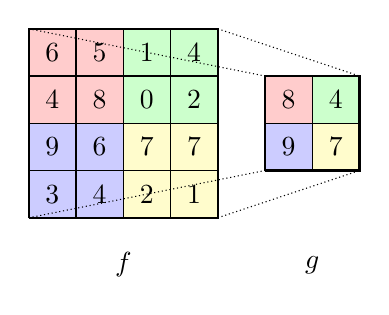
\begin{tikzpicture}[scale=0.6]
    \filldraw[color=blue, opacity=0.2] (0,0) rectangle (2,2);
    \filldraw[color=red, opacity=0.2] (0,2) rectangle (2,4);
    \filldraw[color=green, opacity=0.2] (2,2) rectangle (4,4);
    \filldraw[color=yellow, opacity=0.2] (2,0) rectangle (4,2);

    \filldraw[color=blue, opacity=0.2] (5,1) rectangle (6,2);
    \filldraw[color=red, opacity=0.2] (5,2) rectangle (6,3);
    \filldraw[color=green, opacity=0.2] (6,2) rectangle (7,3);
    \filldraw[color=yellow, opacity=0.2] (6,1) rectangle (7,2);

	\draw [thick] (0,0) -- (0,4) -- (4,4) -- (4,0) -- (0,0);
    \draw (0,1) -- (4,1);
    \draw (0,2) -- (4,2);
    \draw (0,3) -- (4,3);
    \draw (1,0) -- (1,4);
    \draw (2,0) -- (2,4);
    \draw (3,0) -- (3,4);
    \node at (0.5, 0.5) {3};
    \node at (1.5, 0.5) {4};
    \node at (2.5, 0.5) {2};
    \node at (3.5, 0.5) {1};
    \node at (0.5, 1.5) {9};
    \node at (1.5, 1.5) {6};
    \node at (2.5, 1.5) {7};
    \node at (3.5, 1.5) {7};
    \node at (0.5, 2.5) {4};
    \node at (1.5, 2.5) {8};
    \node at (2.5, 2.5) {0};
    \node at (3.5, 2.5) {2};
    \node at (0.5, 3.5) {6};
    \node at (1.5, 3.5) {5};
    \node at (2.5, 3.5) {1};
    \node at (3.5, 3.5) {4};
    
    \draw[densely dotted] (0,0) -- (5,1);
    \draw[densely dotted] (0,4) -- (5,3);
    \draw[densely dotted] (4,4) -- (7,3);
    \draw[densely dotted] (4,0) -- (7,1);
    
    \draw [thick] (5,1) -- (5,3) -- (7,3) -- (7,1) -- (5,1);
    \draw (6,1) -- (6,3);
    \draw (5,2) -- (7,2);
    
    \node at (5.5, 1.5) {9};
    \node at (6.5, 1.5) {7};
    \node at (5.5, 2.5) {8};
    \node at (6.5, 2.5) {4};
    
    \node at (2, -1) {$f$};
    \node at (6, -1) {$g$};
\end{tikzpicture}
    \vspace*{1mm}
    \caption{2D Max-pooling}
    \end{subfigure}
    ~
    \begin{subfigure}[t]{0.55\textwidth}
        \centering
        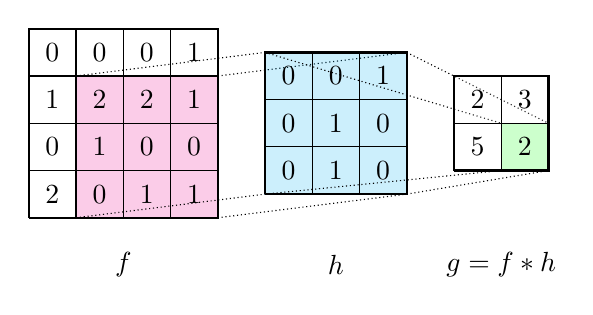
\begin{tikzpicture}[scale=0.6]
    \filldraw[color=magenta, opacity=0.2] (1,0) rectangle (4,3);

	\draw [thick] (0,0) -- (0,4) -- (4,4) -- (4,0) -- (0,0);
    \draw (0,1) -- (4,1);
    \draw (0,2) -- (4,2);
    \draw (0,3) -- (4,3);
    \draw (1,0) -- (1,4);
    \draw (2,0) -- (2,4);
    \draw (3,0) -- (3,4);
    
    \node at (0.5, 0.5) {2};
    \node at (1.5, 0.5) {0};
    \node at (2.5, 0.5) {1};
    \node at (3.5, 0.5) {1};
    \node at (0.5, 1.5) {0};
    \node at (1.5, 1.5) {1};
    \node at (2.5, 1.5) {0};
    \node at (3.5, 1.5) {0};
    \node at (0.5, 2.5) {1};
    \node at (1.5, 2.5) {2};
    \node at (2.5, 2.5) {2};
    \node at (3.5, 2.5) {1};
    \node at (0.5, 3.5) {0};
    \node at (1.5, 3.5) {0};
    \node at (2.5, 3.5) {0};
    \node at (3.5, 3.5) {1};
    
    \draw[densely dotted] (1,0) -- (5,0.5);
    \draw[densely dotted] (1,3) -- (5,3.5);
    \draw[densely dotted] (4,3) -- (8,3.5);
    \draw[densely dotted] (4,0) -- (8,0.5);
    
    \filldraw[color=cyan, opacity=0.2] (5,0.5) rectangle (8,3.5);
    
    \draw [thick] (5,0.5) -- (5,3.5) -- (8,3.5) -- (8,0.5) -- (5,0.5);
    \draw (5,2.5) -- (8,2.5);
    \draw (5,1.5) -- (8,1.5);
    \draw (6,0.5) -- (6,3.5);
    \draw (7,0.5) -- (7,3.5);
    
    \node at (5.5, 1) {0};
    \node at (6.5, 1) {1};
    \node at (7.5, 1) {0};
    \node at (5.5, 2) {0};
    \node at (6.5, 2) {1};
    \node at (7.5, 2) {0};
    \node at (5.5, 3) {0};
    \node at (6.5, 3) {0};
    \node at (7.5, 3) {1};
    
    \draw[densely dotted] (5,0.5) -- (10, 1);
    \draw[densely dotted] (5,3.5) -- (10, 2);
    \draw[densely dotted] (8,3.5) -- (11, 2);
    \draw[densely dotted] (8,0.5) -- (11, 1);
    
    \filldraw[color=white, opacity=0.2] (9,1) rectangle (10,2);
    \filldraw[color=white, opacity=0.2] (9,2) rectangle (10,3);
    \filldraw[color=green, opacity=0.2] (10,1) rectangle (11,2);
    \filldraw[color=white, opacity=0.2] (10,2) rectangle (11,3);
    
    \draw [thick] (9,1) -- (9,3) -- (11,3) -- (11,1) -- (9,1);
    \draw (10,1) -- (10,3);
    \draw (9,2) -- (11,2);
    
    \node at (9.5, 1.5) {5};
    \node at (10.5, 1.5) {2};
    \node at (9.5, 2.5) {2};
    \node at (10.5, 2.5) {3};
    
    \node at (2, -1) {$f$};
    \node at (6.5, -1) {$h$};
    \node at (10, -1) {$g=f\ast h$};
\end{tikzpicture}
        \vspace*{1mm}
        \caption{2D Convolution}
    \end{subfigure}
    \caption{Illustrations of the 2D max-pooling and convolution operations. \textbf{(a)} The max-pooling operation shown takes an input image $f$ and uses a $2\times 2$ filter and stride of two to produce the output image $g$. Note that the maximum value in each coloured region of the input is the resulting value of the corresponding regions of the output. \textbf{(b)} The convolution operation shown takes an input image $f$ and uses a $3\times 3$ kernel $h$ with a stride of one to produce the output image $g=f\ast h$, where $\ast$ denotes the convolution operation. Note that the kernel shown in the convolution operation is ``flipped'' in both the $x$ and $y$ axes before the element-wise multiplication and summation takes place.}
    \label{fig:operations}
\end{figure}

Another feature of CNNs that set them apart from their fully connected counterparts is the localised ``receptive fields'' of the neurons present in convolutional layers. Whilst neurons present in a fully connected layer can receive input from every neuron in the previous layer, neurons present in a convolutional layer can only receive input from a small amount of neighbouring neurons in the previous layer. For example, if a $3\times 3$ kernel is used, a neuron's activation can only be influenced by nine neurons in the previous layer. This area of input that can influence a neuron is called its receptive field. This is one of the reasons why during hyper parameter optimisation, kernel sizes from various layers may be tuned in order to increase or decrease the size of neurons' receptive fields. Hyper parameter optimisation is discussed in Section \ref{sec:hyperparam}.

\subsection{Backpropagation}
\label{sec:backprop}

First popularised by Rumelhart et al. in 1986~\cite{rumelhart}, the backpropagation algorithm is still the main learning mechanism used in neural networks today. Once a loss function is defined to measure the performance of the network, backpropagation can be used to compute the derivative of the loss function with respect to each weight in the network using the chain rule. The derivatives are calculated one layer at a time, iterating backward from the output layer. Since the backpropagation algorithm makes use of the chain rule, the loss function must be differentiable. This must also be the case for the chosen activation functions for each neuron.

An optimisation algorithm can then use these computed derivatives to adjust each weight in order to minimise the chosen loss function. Loss functions used throughout this project are discussed in Section \ref{sec:loss}.

\subsection{Optimisation Algorithms}

Once the derivatives\textemdash or ``gradients''\textemdash have been calculated, an optimisation algorithm is used to determine the exact value each weight should be updated to. When training deep neural networks, some variant of the gradient descent algorithm is often used. Gradient descent~\cite[p. 536]{gradient} is an iterative algorithm designed to find local minima of some differentiable function\textemdash in this case, the loss function. A visualisation of the gradient descent algorithm is shown in Figure \ref{fig:gd}. The gradient descent algorithm evaluates the loss function over the entire dataset before taking a ``step'' in the direction of the gradient computed. A step consists of updating the value of every weight in order to decrease the average loss value that would be achieved by the network when processing the dataset. Evaluating the loss function over the entire dataset once is referred to as an ``epoch''.

The size of the weight update is not only determined by the gradient calculated, but also by a hyper parameter called the ``learning rate''. For example, gradient descent calculates the update for a single weight $w$ as

\begin{equation}
    w := w - \eta\nabla\ell(w)
\end{equation}

\noindent
where $\eta$ is the learning rate and $\nabla\ell(w)$ is the derivative of the loss function $\ell$ with respect to $w$. Choosing an appropriate learning rate is challenging but is essential to allow an optimisation algorithm to converge to a local minimum. A learning rate that is too large can cause the loss function to fluctuate around the minimum, impeding convergence or even causing divergence. The learning rate hyper parameter has a significant effect on training and is one of the most important parameters tuned in the hyper parameter optimisation process (see Section \ref{sec:hyperparam}).


\subsubsection{Stochastic Gradient Descent}

Issues arise when using gradient descent with larger datasets, as evaluating the loss function over the entire dataset before a step can be taken becomes increasingly computationally costly~\cite{gdbad}. These issues have given rise to the popularity of the stochastic gradient descent (SGD) and the mini-batch gradient descent optimisation algorithms. SGD is a variant of the gradient descent algorithm that takes a step each time a sample is processed rather than only once the entire dataset is processed. Mini-batch gradient descent is yet another variant of gradient descent in which weights are updated after evaluating the loss function over a subset\textemdash or ``batch''\textemdash of the training samples.

\begin{figure}[t]
    \centering
    \begin{tikzpicture}[scale=1.1]
	\begin{axis}[
% 	colormap/greenyellow,
	colormap name=cool2,
% 	view={0}{90}
	xlabel=$x$,
	ylabel=$y$,
	zlabel=Loss,
	zmin=0.1, zmax=1.9,
	xtick distance=175,
	ytick distance=175,
	xticklabels=\empty,
	yticklabels=\empty,
	zticklabels=\empty
	]
% 	\addplot3[surf,
% 		domain=0:360,samples=40] 
% 		{0.5*sin(x-100)*sin(y-50) - 0.000005*((x-100)^2) + 0.000005*((y-50)^2) + 1};
    \addplot3 [surf, mesh/rows=36] table [x=xs, y=ys, z=zs, col sep=comma] {csv/surf.csv};
    
	\addplot3 [black, mark=*, line width=0.8pt, mark size=0.8pt] table [x=xs, y=ys, z=zs, col sep=comma] {csv/sgd.csv};
	
% 	\addplot3 [black, mark=*, line width=0.8pt, mark size=0.8pt] table [x=xs, y=ys, z=zs, col sep=comma] {csv/sgd2.csv};
	
	\addplot3 [black, mark=*, line width=0.8pt, mark size=0.8pt] table [x=xs, y=ys, z=zs, col sep=comma] {csv/sgd3.csv};
	
	\node[] at (axis cs: 320, 200, 1.9) {\scriptsize{($x_0, y_0, \ell(x_0, y_0)$)}};
	
	\node[] at (axis cs: 260, 200, 0.1) {\scriptsize{($x_n, y_n, \ell(x_n, y_n)$)}};
	\end{axis}
\end{tikzpicture}
    \caption{A diagram visualising the gradient descent algorithm for a model containing two trainable parameters, $x$ and $y$. Given a random starting configuration with parameters $x_0$ and $y_0$, the average loss value that would be achieved when processing the entire dataset is given by $\ell(x_0, y_0)$. Say gradient descent takes $n$ steps in the direction of steepest descent at each iteration until the loss value converges to some local minimum, $x_n$ and $y_n$ would be the final parameter values and the final loss would be $\ell(x_n, y_n)$. It is worth noting that even though the two starting configurations shown in the diagram both converge to the same local minimum, this might not always be the case. A starting configuration nearer to one of the other possible local minima would most likely not converge to the example local minimum $\ell(x_n, y_n)$ shown.}
    \label{fig:gd}
\end{figure}

\subsubsection{Adam}

First introduced by Kingma and Ba in 2014, Adam~\cite{adam} is an optimisation algorithm that is also based off of SGD. However, rather than using the same learning rate across all parameters, Adam computes individual adaptive learning rates for different parameters. These individual learning rates are based off of estimates of the first moment (the mean) and second moment (the uncentered variance) of the gradients~\cite{gdbad}. Kingma and Ba showed empirically that Adam works well in practice and compares favourably to other optimisation algorithms when optimising both fully connected ANNs and deep CNNs.

\subsection{Loss functions}
\label{sec:loss}

A loss function takes both the actual and predicted values of a training sample, and outputs some measure of how well a model performed by producing that prediction. As mentioned in Section \ref{sec:backprop}, backpropagation makes use of the derivative of the loss function with respect to each parameter in order to minimise the loss achieved. If the appropriate loss function is chosen, minimising the loss should improve the performance achieved by the network. It is for this reason that loss functions must be differentiable. The loss functions that were experimented with throughout this project are outlined below.

\subsubsection{Binary Cross-Entropy Loss}

\begin{equation}
    L(y, \hat{y})=-\frac{1}{N} \sum_{i=0}^{N}\left(y * \log \left(\hat{y}_{i}\right)+(1-y) * \log \left(1-\hat{y}_{i}\right)\right)
\end{equation}

where $y$ is the actual value, and $\hat{y}$ is the predicted value.

\subsubsection{Focal Loss}

\begin{equation}
    \mathrm{FL}\left(p_{\mathrm{t}}\right)=-\left(1-p_{\mathrm{t}}\right)^{\gamma} \log \left(p_{\mathrm{t}}\right)
\end{equation}

~\cite{focalloss}

\subsubsection{Dice coefficient}

\subsection{Accuracy Metrics}

Although loss functions can be used to measure performance, their main purpose is to be used to train the network. To quantify the performance achieved by a network, an accuracy metric should instead be used. Accuracy metrics do not play a direct role in training networks, though they can be used indirectly\textemdash for example, to determine whether or not to continue training. Choosing an appropriate accuracy metric is essential and proved challenging throughout this project. The main accuracy metric decided upon was based off of the Hausdorff distance discussed in Section \ref{sec:hausdorff}.

\subsection{Datasets}

Introduce train test val split and what they are all used for.

Referred to as a ``beautiful free lunch'' by Geoffrey Hinton~\cite[p. 141]{earlystopping}, early stopping is.

\subsection{Pooling}

\subsection{Overfitting}

The term overfitting is used to describe when a model performs well on the data on which it is trained, yet poorly on data which it has not yet been exposed to.

\subsubsection{Data augmentation}

Data augmentation is the process of augmenting the labelled training data in some way in order to increase the amount of training data available. This augmentation can be performed ``online'' with each training sample being randomly augmented during the training process, or it can be performed ``offline'' with the augmentation taking place before training. The training data can be augmented in many ways. Common examples for 2D images are: random rotations within some predefined range, random changes to brightness levels, and random horizontal and vertical flips. Data augmentation is used to reduce overfitting.

\subsubsection{Dropout}

Another technique often used to reduce overfitting, is ``dropout''.

\subsection{Hyper parameter optimisation}
\label{sec:hyperparam}

Define what a parameter and hyper parameter is. Talk about diff algorithms (genetic vs brute force).

\subsection{SegNet}

Mention that segnet and unet are both fully convolutional so no dense layers (fully connected)

\subsection{U-Net}

Presented by Ronneberger et al. in 2015~\cite{ronneberger2015u}, U-Net is a convolutional neural network architecture that was initially used to perform instance segmentation on biomedical images, but has since been used on a wider range of visual data. The U-Net architecture consists of three sections: the contracting path, the bottleneck, and the expanding path. The contracting path follows the typical architecture of a convolutional network, in that the image is gradually downsampled and the number of feature channels is increased. The expansion path then gradually reconstructs the image via `up-convolutions'. Throughout the expansion path, the feature channels from the corresponding contraction layers are appended to the feature channels in the expansion layers. This allows the features that are learned whilst contracting the image to also be used to reconstruct it. A diagram of the U-Net architecture is shown in Figure~\ref{fig:unet}.

\begin{figure}[t]
    \centering
    \includegraphics[width=1\textwidth]{images/U-Net.pdf}
    \caption{A diagram of the U-Net architecture. Each cube represents a layer. The orange cubes represent convolutional layers, the red cubes represent max-pooling, and the blue cubes represent up-convolutions. The green arrows represent the feedforward of information from one layer to the next, whereas the blue arrows represent the concatenation of the feature maps of one layer to another.}
    \label{fig:unet}
\end{figure}

\subsection{CycleGANs and pix2pix}

Throughout this project, various deep learning techniques are utilised in an attempt to maximise the performance achieved.

\section{Classical Image Processing Techniques}

\subsection{Hausdorff distance}
\label{sec:hausdorff}

\section{Related Work}

% -----------------------------------------------------------------------------

\chapter{Project Execution}
\label{chap:execution}

\section{Two Dimensional Boundary Extraction}

\subsection{Labelling the Data}

\subsection{Dataset Curation}

\subsubsection{Splitting the Dataset}

\subsection{Architecture}

\subsection{Data Augmentation}

\subsection{Early Stopping}

\section{Three Dimensional Boundary Extraction}

\subsection{Dataset Expansion}

\subsection{Architecture Modification}

\subsection{Data Loader Implementation}

\subsection{Three Dimensional Data Augmentation}

\section{Accuracy Metric Implementation}

\subsection{Skeletonisation}

(Show algorithm and maybe some source code?)

\subsection{The \texttt{ctypes} Module}

\section{Density Band Width Estimation}

\subsection{Point Sampling}

% {\bf A topic-specific chapter, of roughly $15$ pages} 
% \vspace{1cm} 

% \noindent
% This chapter is intended to describe what you did: the goal is to explain
% the main activity or activities, of any type, which constituted your work 
% during the project.  The content is highly topic-specific, but for many 
% projects it will make sense to split the chapter into two sections: one 
% will discuss the design of something (e.g., some hardware or software, or 
% an algorithm, or experiment), including any rationale or decisions made, 
% and the other will discuss how this design was realised via some form of 
% implementation.  

% This is, of course, far from ideal for {\em many} project topics.  Some
% situations which clearly require a different approach include:

% \begin{itemize}
% \item In a project where asymptotic analysis of some algorithm is the goal,
%       there is no real ``design and implementation'' in a traditional sense
%       even though the activity of analysis is clearly within the remit of
%       this chapter.
% \item In a project where analysis of some results is as major, or a more
%       major goal than the implementation that produced them, it might be
%       sensible to merge this chapter with the next one: the main activity 
%       is such that discussion of the results cannot be viewed separately.
% \end{itemize}

% \noindent
% Note that it is common to include evidence of ``best practice'' project 
% management (e.g., use of version control, choice of programming language 
% and so on).  Rather than simply a rote list, make sure any such content 
% is useful and/or informative in some way: for example, if there was a 
% decision to be made then explain the trade-offs and implications 
% involved.

% \section{Example Section}

% This is an example section; 
% the following content is auto-generated dummy text.
% \lipsum

% \subsection{Example Sub-section}

% \begin{figure}[t]
% \centering
% foo
% \caption{This is an example figure.}
% \label{fig}
% \end{figure}

% \begin{table}[t]
% \centering
% \begin{tabular}{|cc|c|}
% \hline
% foo      & bar      & baz      \\
% \hline
% $0     $ & $0     $ & $0     $ \\
% $1     $ & $1     $ & $1     $ \\
% $\vdots$ & $\vdots$ & $\vdots$ \\
% $9     $ & $9     $ & $9     $ \\
% \hline
% \end{tabular}
% \caption{This is an example table.}
% \label{tab}
% \end{table}

% \begin{algorithm}[t]
% \For{$i=0$ {\bf upto} $n$}{
%   $t_i \leftarrow 0$\;
% }
% \caption{This is an example algorithm.}
% \label{alg}
% \end{algorithm}

% \begin{lstlisting}[float={t},caption={This is an example listing.},label={lst},language=C]
% for( i = 0; i < n; i++ ) {
%   t[ i ] = 0;
% }
% \end{lstlisting}

% This is an example sub-section;
% the following content is auto-generated dummy text.
% Notice the examples in Figure~\ref{fig}, Table~\ref{tab}, Algorithm~\ref{alg}
% and Listing~\ref{lst}.
% \lipsum

% \subsubsection{Example Sub-sub-section}

% This is an example sub-sub-section;
% the following content is auto-generated dummy text.
% \lipsum

% \paragraph{Example paragraph.}

% This is an example paragraph; note the trailing full-stop in the title,
% which is intended to ensure it does not run into the text.

% -----------------------------------------------------------------------------

\chapter{Critical Evaluation}
\label{chap:evaluation}

\section{Comparisons with Existing Techniques}

\section{Future Work}

% {\bf A topic-specific chapter, of roughly $15$ pages} 
% \vspace{1cm} 

% \noindent
% This chapter is intended to evaluate what you did.  The content is highly 
% topic-specific, but for many projects will have flavours of the following:

% \begin{enumerate}
% \item functional  testing, including analysis and explanation of failure 
%       cases,
% \item behavioural testing, often including analysis of any results that 
%       draw some form of conclusion wrt. the aims and objectives,
%       and
% \item evaluation of options and decisions within the project, and/or a
%       comparison with alternatives.
% \end{enumerate}

% \noindent
% This chapter often acts to differentiate project quality: even if the work
% completed is of a high technical quality, critical yet objective evaluation 
% and comparison of the outcomes is crucial.  In essence, the reader wants to
% learn something, so the worst examples amount to simple statements of fact 
% (e.g., ``graph X shows the result is Y''); the best examples are analytical 
% and exploratory (e.g., ``graph X shows the result is Y, which means Z; this 
% contradicts [1], which may be because I use a different assumption'').  As 
% such, both positive {\em and} negative outcomes are valid {\em if} presented 
% in a suitable manner.

% -----------------------------------------------------------------------------

\chapter{Conclusion}
\label{chap:conclusion}

% {\bf A compulsory chapter,     of roughly $5$ pages} 
% \vspace{1cm} 

% \noindent
% The concluding chapter of a dissertation is often underutilised because it 
% is too often left too close to the deadline: it is important to allocation
% enough attention.  Ideally, the chapter will consist of three parts:

% \begin{enumerate}
% \item (Re)summarise the main contributions and achievements, in essence
%       summing up the content.
% \item Clearly state the current project status (e.g., ``X is working, Y 
%       is not'') and evaluate what has been achieved with respect to the 
%       initial aims and objectives (e.g., ``I completed aim X outlined 
%       previously, the evidence for this is within Chapter Y'').  There 
%       is no problem including aims which were not completed, but it is 
%       important to evaluate and/or justify why this is the case.
% \item Outline any open problems or future plans.  Rather than treat this
%       only as an exercise in what you {\em could} have done given more 
%       time, try to focus on any unexplored options or interesting outcomes
%       (e.g., ``my experiment for X gave counter-intuitive results, this 
%       could be because Y and would form an interesting area for further 
%       study'' or ``users found feature Z of my software difficult to use,
%       which is obvious in hindsight but not during at design stage; to 
%       resolve this, I could clearly apply the technique of Smith [7]'').
% \end{enumerate}

% =============================================================================

% Finally, after the main matter, the back matter is specified.  This is
% typically populated with just the bibliography.  LaTeX deals with these
% in one of two ways, namely
%
% - inline, which roughly means the author specifies entries using the 
%   \bibitem macro and typesets them manually, or
% - using BiBTeX, which means entries are contained in a separate file
%   (which is essentially a databased) then inported; this is the 
%   approach used below, with the databased being dissertation.bib.
%
% Either way, the each entry has a key (or identifier) which can be used
% in the main matter to cite it, e.g., \cite{X}, \cite[Chapter 2}{Y}.

\backmatter

\bibliography{dissertation}

% -----------------------------------------------------------------------------

% The dissertation concludes with a set of (optional) appendicies; these are 
% the same as chapters in a sense, but once signaled as being appendicies via
% the associated macro, LaTeX manages them appropriatly.

\appendix

\chapter{An Example Appendix}
\label{appx:example}

Content which is not central to, but may enhance the dissertation can be 
included in one or more appendices; examples include, but are not limited
to

\begin{itemize}
\item lengthy mathematical proofs, numerical or graphical results which 
      are summarised in the main body,
\item sample or example calculations, 
      and
\item results of user studies or questionnaires.
\end{itemize}

\noindent
Note that in line with most research conferences, the marking panel is not
obliged to read such appendices.

% =============================================================================
